\documentclass[10pt,twocolumn]{article}
\usepackage[a4paper,margin=0.8in,columnsep=0.25in]{geometry}
\usepackage{graphicx}
\usepackage{booktabs}
\usepackage{url}
\usepackage{microtype}
\usepackage{titlesec}
\titlespacing*{\section}{0pt}{1.0ex}{0.5ex}
\titleformat*{\section}{\normalsize\bfseries}
\setlength{\parskip}{0.3ex}

\title{A Pilot Test of LLM-Driven Patch Search on the FIT SDK Decoder}
\author{Rrraaaeee}
\date{}

\begin{document}
\maketitle

\begin{abstract}
We built an evolutionary search that asks a language model to rewrite functions of
the FIT SDK 21.201.0 decoder, and calibrated its decision rule on libraries of known
speed. \textbf{This is a pilot with a negative result: no search run confirmed a
speedup, and the search did not beat calling the model with no feedback.} Three
search runs and three no-feedback runs of 10 calls each confirmed nothing. A single
\texttt{-O3} flag gave about 10\%. On our loaded, non-reference machine the rule
made 0 false claims in 30 null trials, consistent with a true rate up to 11.6\%, but
caught a true 10\% speedup only 7 times in 10. The best candidate, from a
no-feedback run, measured about 3\% faster when re-measured after the fact. We treat
that as a lead, not a result.
\end{abstract}

\section{What we built}
\textbf{Search.} Each individual is a unified diff against the stock SDK. A
generation picks a parent by a tournament of two, draws one function body, asks the
model for a rewrite, splices it, and has the provided harness compile the patched
tree, check correctness and time it against the reference. Compile and correctness
failures go into the next prompt. A reply identical to its input is logged and not
measured. The population keeps 6 patches. The best-of-N control (C3) uses the same
code, but every call starts from the unmodified baseline with no feedback.

\textbf{Decision rule.} The rule reads only the raw \texttt{timings} from
\texttt{measure-patch --no-decision}. For each process it divides the candidate's
median per-repetition time by the reference's, and takes the median of those ratios
over the 10 processes. It calls a candidate faster when all three hold: (1) that
ratio is below 0.98, (2) an exact two-sided sign-flip test over the per-process
log-ratios gives $p<0.01$, and (3) the largest and smallest per-process ratios
differ by at most 0.25. A candidate that is significant or unstable is measured a
second time; acceptance needs both measurements to pass, and the higher ratio is
kept. Calibration calls this same code through a \texttt{--judge} mode. The
thresholds were fixed before Phase 0 and not changed afterwards. The rule assumes
exchangeable processes, not independent repetitions.

\section{Setup and deviations}
All numbers come from one machine, \texttt{leffe2}: two Xeon Gold 6242R CPUs (80
logical CPUs), g++ 15.2.0, \texttt{-O2}, \texttt{--repeat 10}, \texttt{--repetitions
9}. The machine was shared. Load averages we observed ranged from 13 to 97, and CPU
frequency scaling was on. The search model was \texttt{claude-haiku-5-5} through the
Claude Messages API, default sampling, seeds 1--3; a separate test call to that
model reported the same id. A decode reads 907,007 bytes, 34,251 messages and
428,714 fields, with checksum \texttt{92bebfd7f8978fc8}. The null run from
\texttt{init} gave ratio 0.9997 (spread 0.017), with a 269.87\,ms baseline.

The pilot departs from the assignment in these ways. Results are not comparable
with Xeon \texttt{xcnc}/\texttt{xcnd} measurements.
\begin{itemize}\setlength{\itemsep}{0pt}
\item Everything ran on \texttt{leffe2}, not the required cluster nodes.
\item Each configuration had 3 seeds of 10 generations, not at least 5 seeds (C4)
and 40 generations.
\item \texttt{perf} is not installed, so regions were not profile-guided. We drew
uniformly from 155 functions in three decoder files chosen by hand
(\texttt{fit\_decode}, \texttt{fit\_mesg}, \texttt{fit\_field\_base}).
\item \textbf{The human control (C2) was not run.}
\item Each of the six pilot runs reached a clean null only on its third
\texttt{init} attempt, probably because six builds ran concurrently. Keeping the first clean
attempt selects for a favourable null, so those nulls are weaker evidence.
\end{itemize}

\section{Phase 0: calibration}
We ran 80 trials interleaved round by round, at each pair's \texttt{min\_time} chosen
by \texttt{CanMehCalibrate} (0.033--0.038\,s) and 20,000 reference work units, under
load 28--34. \texttt{CanMehCalibrate} passed its five required rows and refused
\texttt{broken-digest} at stage \texttt{correctness} and
\texttt{shared-install-name} at stage \texttt{load}.

\begin{table}[t]
\centering\footnotesize
\begin{tabular}{@{}lrrcrr@{}}
\toprule
Pair & True & Faster & 95\% CI & Median & Bias\\
\midrule
null & 1.0000 & 0/30 & 0--.116 & 1.0066 & +.0068\\
faster 1\% & 0.9900 & 0/10 & 0--.308 & 0.9945 & +.0049\\
faster 2\% & 0.9804 & 2/10 & .025--.556 & 0.9758 & $-$.0013\\
faster 5\% & 0.9524 & 4/10 & .122--.738 & 0.9563 & +.0038\\
faster 10\% & 0.9091 & 7/10 & .348--.933 & 0.9096 & +.0019\\
slower 10\% & 1.1000 & 0/10 & 0--.308 & 1.1039 & +.0044\\
\bottomrule
\end{tabular}
\caption{The rule on calibration pairs. CI is Clopper--Pearson~\cite{cp}.
Bias is the mean reported ratio minus the true ratio.}
\label{tab:cal}
\end{table}

\begin{figure}[t]
\centering
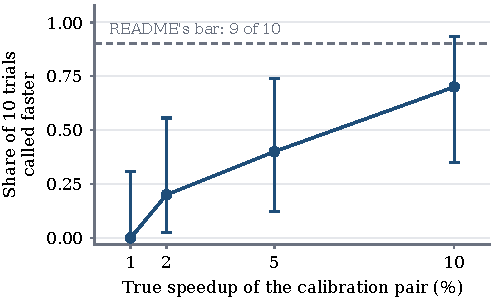
\includegraphics[width=\columnwidth]{figures/detection.pdf}
\caption{Detection rate by true effect, with 95\% Clopper--Pearson intervals. No
effect reached 9 of 10.}
\label{fig:det}
\end{figure}

Table~\ref{tab:cal} and Figure~\ref{fig:det} give the three numbers.
\textbf{False-positive rate:} 0 of 30, which supports only a rate below 11.6\%.
\textbf{Detection threshold:} above 10\% at these settings; no tested effect reached
9 of 10. With 10 trials each, the intervals overlap heavily, and the curve shows only
a rising trend. The 2\% pair sits on the rule's 2\% floor, so a rate near one half
would be expected there at best. \textbf{Bias:} the mean error is at most 0.7\% in
magnitude and positive at five of six settings, though single null trials ranged
from 0.968 to 1.063. Per-process ratios typically spread by 0.12--0.21, more than
the effects under test.

Lag-1 autocorrelation of \texttt{candidate\_ns} had trial-level medians of $-0.03$ to
$-0.14$ on the calibration loop, about what 9-point series show by chance, and 0.004
(process range $-0.19$ to 0.60) in one SDK measurement. One measurement cannot
characterize the SDK decoder. These pairs scale the whole workload uniformly and
differ from the SDK's timing behaviour, so the threshold does not transfer to real
patches.

\textbf{Inert patch.} A comment spliced into \texttt{Decode::Decode} measured ratio
1.012, $p=0.27$, and was not called faster. Its spread of 0.36 flagged it unstable.

\section{Phase 1: search and controls}
\begin{table}[t]
\centering\footnotesize
\begin{tabular}{@{}lrrrrr@{}}
\toprule
Run & Meas. & Lowest ratio & Unst. & Conf. & Tokens\\
\midrule
search 1 & 10 & 0.9949 & 6 & 0 & 16,418\\
search 2 & 9 & 0.9957 & 5 & 0 & 18,567\\
search 3 & 10 & 0.9924 & 3 & 0 & 15,378\\
best-of-N 1 & 10 & 0.9627 & 5 & 0 & 17,178\\
best-of-N 2 & 10 & 0.9945 & 2 & 0 & 16,174\\
best-of-N 3 & 9 & 0.9970 & 2 & 0 & 19,395\\
\bottomrule
\end{tabular}
\caption{Pilot runs, 10 model calls each. \emph{Meas.}: candidates measured.
\emph{Lowest ratio}: lowest kept ratio, not a confirmed speedup. \emph{Unst.}: runs
flagged unstable. \emph{Conf.}: confirmed.}
\label{tab:runs}
\end{table}

Table~\ref{tab:runs} summarizes the 60 model calls, which used 103,110 tokens
and took 1,116--1,637\,s per run. Of those calls, 58 candidates were measured, one
failed to compile, and one reply held no usable code. Twenty-three measurements were
unstable. \texttt{best\_confirmed\_speedup} is 1.0 in every run, so the bonus quotient
is zero.

\textbf{C3 and C4.} At an equal call budget, the search's best retained speedups
were median 1.0051 (range 1.0043--1.0076), and best-of-N's were median 1.0056 (range
1.0030--1.0387). Neither arm confirmed anything. We see no evidence that selection
and feedback helped, but 3 seeds of 10 calls cannot show they do not. Lowest retained
ratios are also biased downward by selection and should not be read as speedups.

\textbf{C1.} We timed each build against the \texttt{-O2} reference in one process,
three trials each. \texttt{-O3} gave ratios 0.900, 0.906 and 0.916; two of the three
passed the rule and one was unstable. \texttt{-O3 -march=native} gave 0.927, 0.936
and 0.925; one passed. Its \texttt{init} null failed (ratio 1.020, spread 0.75), as
did \texttt{-O3}'s, so we weight these as indicative. The roughly 10\% from
\texttt{-O3} exceeded every candidate retained in either arm, and a compiler
preserves observable behaviour by construction.

\textbf{Follow-up on the best candidate.} Best-of-N 1, generation 2, changed the
\texttt{FieldBase} copy constructor to initialize its two vectors in the member
initializer list rather than assigning them in the body. In its run, both
measurements had $p<0.01$ and the kept ratio was 0.9627, but the rule rejected it
for a spread of 0.40. We then measured it three more times: ratios 0.9668, 0.9695
and 0.9682. Two passed the rule; the third was unstable, with $p=0.96$. Our
modification therefore made the decode about 3\% faster in those measurements. We
chose this candidate after seeing all results, on a noisy machine and with a rule
whose detection is weak at this size, so it needs confirming on a reference node. We
did not profile it; avoiding default construction followed by assignment is our
hypothesis for the mechanism.

\section{What we believe, and what we do not}
We believe the measurement path works: inert and null measurements were not called
faster, and known ratios were recovered with small bias. We believe a compiler flag
beat everything the pilot's search kept. We do not claim the search or the model
produced a confirmed speedup, that selection adds nothing, or that the 3\% lead is
real. The pilot's small budget, hand-picked regions, weaker model and noisy host all
limit it. A full study needs the reference nodes, 5 or more seeds of 40 generations,
profile-guided regions and the human control.

\textbf{Abandoned runs.} A 5-generation test preceded the pilot. Four of its five
replies changed nothing, because our prompt allowed that; we removed the allowance
and made unchanged replies skip measurement. Both C1 builds were abandoned in the
main pilot script, the first for a failed null and the second because
\texttt{--opt "-O3 -march=native"} is passed as one flag and does not compile. The
follow-up reused the built \texttt{-O3} library and used a compiler wrapper for
\texttt{-march=native}. All logs are in \texttt{results/}.

\footnotesize
\begin{thebibliography}{9}\setlength{\itemsep}{0pt}
\bibitem{cp} C.~J.~Clopper and E.~S.~Pearson. The use of confidence or fiducial
limits illustrated in the case of the binomial. \emph{Biometrika}, 26(4):404--413, 1934.
\bibitem{sdk} Garmin. FIT C++ SDK, tag 21.201.0.
\url{https://github.com/garmin/fit-cpp-sdk}.
\end{thebibliography}
\end{document}
